\documentclass[10pt,a4paper,ngerman]{article}
\usepackage[margin=2.5cm]{geometry}
\usepackage[T1]{fontenc}
\usepackage[utf8]{inputenc} % Zeichensatz
\usepackage[ngerman]{babel} % Sprachpaket
\usepackage{amsmath}  % Mathematik
\usepackage{amsfonts} % Mathematik
\usepackage{amssymb}  % Mathematik
\usepackage{palatino} % Schriftart
\usepackage{titling}  % für eigene Überschrift
\usepackage{graphicx}
\usepackage{subcaption}
\usepackage{wasysym}  % enthält Symbole, wie Quadrate (für Multiple Choice Fragen)
\usepackage{dirtree}  % Verzeichnisbäume
\usepackage{hyperref} % Hyperlinks und andere Verlinkungen

% Package für die Kopf- und Fußzeilen
\usepackage{scrlayer-scrpage}
\pagestyle{scrheadings}
\clearpairofpagestyles % Die einzelnen Bereiche leeren

% Quelltext-Listings 
\usepackage{listings} % Listings
\usepackage{color}    % Syntax-Highlighting

% Farben definieren (für Syntax-Highlighting)
\definecolor{middlegray}{rgb}{0.5,0.5,0.5}
\definecolor{lightgray}{rgb}{0.8,0.8,0.8}
\definecolor{darkgray}{gray}{0.2} % gray: nur ein Wert wird angegeben, welcher dem Grauton entspricht
\definecolor{comment}{rgb}{0.0,0.5,0.0}
\definecolor{keywordcolor}{rgb}{0.0, 0.28, 0.67}

\newcommand{\lstfs}{\fontsize{10}{12}}

% Listings formatieren
\lstset{
   	basicstyle=\ttfamily\lstfs,
   	keywordstyle=\bfseries\ttfamily\color{keywordcolor},
   	stringstyle=\color{darkgray}\ttfamily,
   	commentstyle=\color{comment}\ttfamily,
  	emph={square}, 
   	emphstyle=\ttfamily,
   	emph={[2]root,base},
   	emphstyle={[2]\ttfamily},
   	showstringspaces=false,
   	flexiblecolumns=false,
   	tabsize=2,
   	numbers=left,
   	numberstyle=\tiny,
   	numberblanklines=false,
   	stepnumber=5,
   	firstnumber=1,
 	numberfirstline=true,
   	numbersep=10pt,
	xleftmargin=15pt,
	literate={ö}{{\"o}}1
           {ä}{{\"a}}1
           {ü}{{\"u}}1
           {ß}{{\ss}}1
}



% Metainformationen
\title{Evaluation -- Praktikum 2}
\author{Die Lokalisatoren}

\ihead{}
\chead{}
\ohead{}
\ifoot{}
\cfoot{\pagemark}
\ofoot{}


\newcommand{\doctitle}[1]{\begin{center}\begin{huge}#1\end{huge}\end{center}}

% 1. Variante des docheader (ohne Parameter)
% dann wird der Autor unter der Überschrift ausgegeben
\newcommand{\docheader}{\doctitle{\thetitle}\begin{center}\theauthor\end{center}\hrule\vspace{1em}}

% 2. Variante des docheader (mit Parameter)
% was im Parameter steht wird unter der Überschrift ausgeben
\newcommand{\docheaderparam}[1]{\doctitle{\thetitle}\begin{center}#1\end{center}\hrule\vspace{1em}}

\newcommand{\timbox}[1]{\begin{center}\fbox{\begin{minipage}[t]{0.8\textwidth}#1\end{minipage}}\end{center}}

\newcommand{\code}[1]{\texttt{#1}}

% Für Multiple Choice
\newcommand{\choice}{\item[\Square]}
\newcommand{\cchoice}{\item[\CheckedBox]} % cc = correc choice

\setlength{\parskip}{0em}
\setlength{\parindent}{0em}
\renewcommand{\baselinestretch}{1.15}

\begin{document}

\docheader

\section{Wie und wo wir messen}

Auf jede Route werden drei verschiedene Verfahren angewandt: 
\begin{itemize}
	\item FusedLocationProvider - \code{PRIORITY\_HIGH\_ACCURACY} (nachfolgend "`FLP\_HIGH"' genannt)
	\item FusedLocationProvider - \code{PRIORITY\_LOW\_POWER} (nachfolgend "`FLP\_LOW"' genannt)
	\item LocationManager - \code{GPS\_PROVIDER} (nachfolgend "`LM\_GPS"' genannt)
\end{itemize}

Dabei entschieden wir uns für FLP\_HIGH, um die genaueste Positionierung zu erhalten. FLP\_LOW verzichte größtenteils auf GPS- und Wi-Fi-Signale und ermittle die Position über Cell Tower (laut Google). LM\_GPS wurde von uns ausgewählt, um die Genauigkeit von GPS zu der höchstmöglichen Genauigkeit und "`Cell Tower-Genauigkeit"' einzuschätzen bzgl. in Relation zu setzen. \\Sowohl die beiden Methoden des Fused-Location-Providers als auch der LocationManager wurden mit einem Update-Intervall von 3 Sekunden versehen. Zudem werden die aufgezeichneten und vordefinierten Routen als Polylines in einer Google Maps Activity eingezeichnet\\

Zur Überprüfung der einzelnen Verfahren wurden zwei Routen definiert (Abbildung \ref{fig:routen}). Das Abgehen einer Route folgt dabei folgendem Schema: An Position des ersten Flags wird der "`Start"'-Button betätigt. Sobald die erste Positionierung erfolgte, wird der "`Timestamp"'-Button betätigt und Route in Schritttempo abgegangen. Jetzt wird der "`Timestamp"'-Button immer betätigt, wenn ein Flag der "`Groundtruth"' passiert wird. Am Ende der Route wird abschließend der "`Timestamp"'- und "`Stop"'-Button betätigt.

\begin{figure}[h!]
	\centering
	\begin{subfigure}[b]{.64\textwidth}
		\centering
        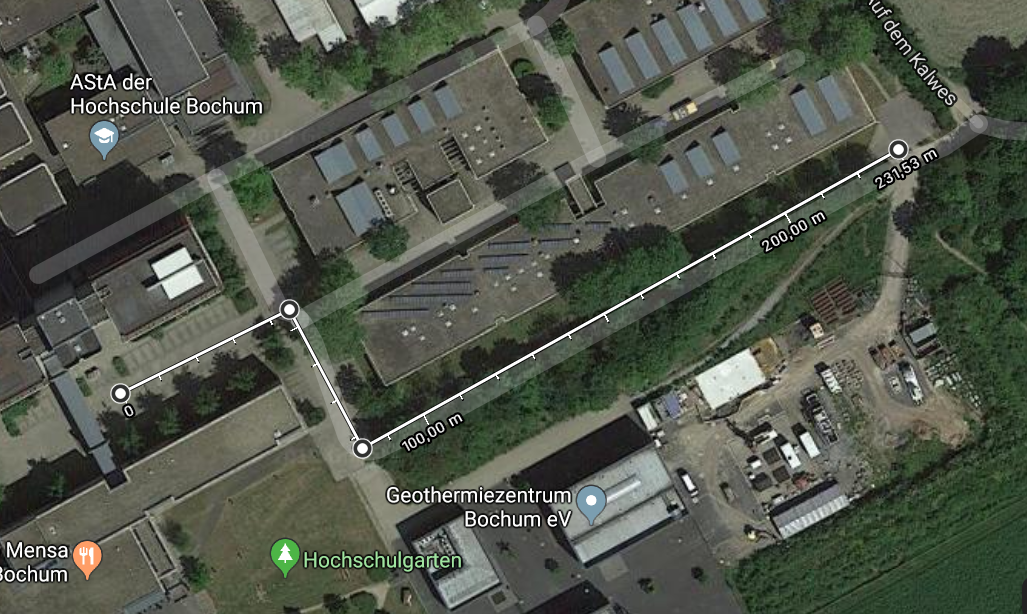
\includegraphics[height=5.2cm]{route1}
        \caption{Route  1 (Outdoors)}
        \label{fig:route1}
    \end{subfigure}
    \begin{subfigure}[b]{.35\textwidth}
    	\centering
        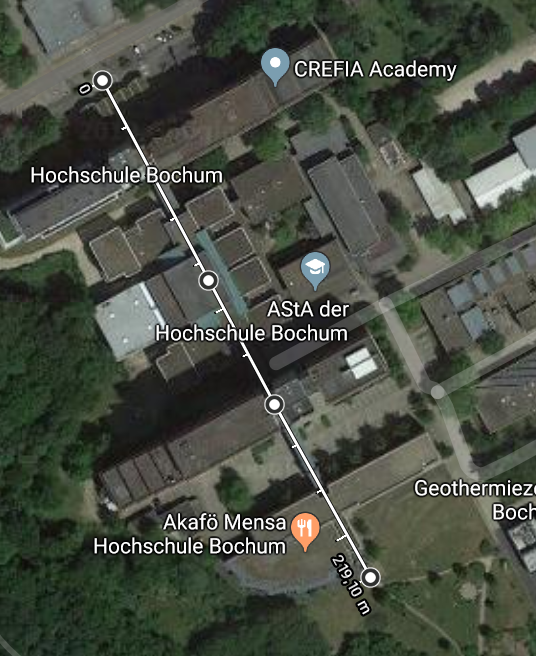
\includegraphics[height=5.2cm]{route2}
        \caption{Route 2 - (Indoors)}
        \label{fig:route2}
    \end{subfigure}
    \caption{Die "`Groundtrouth"' der Routen mit den einzelnen Flags}
    \label{fig:routen}
\end{figure}

\section{Erwartungen}
	
\section{Auswertung}	

\renewcommand{\arraystretch}{1.2}
\begin{table}
	\centering
	\caption{Ergebnisse Route 1 -- Outdoors (Abbildung \ref{fig:route1})}
	\begin{tabular}{|l|l|l|l|}
	\hline
	Fehler (in Meter) & FLP\_HIGH & FLP\_LOW & LM\_GPS \\
	\hline
	\multicolumn{4}{|c|}{\textit{Lagemaße}}\\
	\hline
	Median & $38,593$ & $38,22$ & $74,939$ \\
	Konfidenzlevel 95\% & $120,746$ & $122,055$ & $151,976$ \\
	Arithm. Mittel & $49,431$ & $49,635$ & $84,736$ \\
	\hline
	\multicolumn{4}{|c|}{\textit{Streumaße}}\\
	\hline
	Standardabweichung & $40,274$ & $39,809$ & $45,163$ \\
	\hline
	\end{tabular}
\end{table}

\begin{table}
	\centering
	\caption{Ergebnisse Route 2 -- Indoors (Abbildung \ref{fig:route2})}
	\begin{tabular}{|l|l|l|l|}
	\hline
	Fehler (in Meter) & FLP\_HIGH & FLP\_LOW & LM\_GPS \\
	\hline
	\multicolumn{4}{|c|}{\textit{Lagemaße}}\\
	\hline
	Median & $23,459$ & $26,111$ & $149,883$ \\
	Konfidenzlevel 95\% & $61,455$ & $69,472$ & $200,939$ \\
	Arithm. Mittel & $27,788$ & $29,8$ & $105,941$ \\
	\hline
	\multicolumn{4}{|c|}{\textit{Streumaße}}\\
	\hline
	Standardabweichung & $18,721$ & $21,96$ & $77,317$ \\
	\hline
	\end{tabular}
\end{table}
	
\end{document}